In order to evaluate how the prototype ("'Andromeda"') described in the previous chapter performs when compared to other music library visualizations, a user study has been carried out and analyzed. As the publicly available mobile apps for Android don't support any form of artist discovery, the scope of the user study will be limited to the visualization of artists, and the impact of using Andromeda on usage metrics, as opposed to using other predetermined music apps (visualization methods).

In this Chapter, the conception, execution, and analysis of the user study will be described, in this order:

\begin{itemize}
	\item \textbf {Hypotheses} - Defines a list of 5 hypotheses to be examined by the user study.
	\item \textbf {Metrics and Tools} - Describes how the study will gather which data.
	\item \textbf {Population, Setup, and Process} - Lists execution details of the study, together with a description of the test participants.
	\item \textbf {Results and Data} - Summarizes the gathered data and provides statistical key figures.
	\item \textbf {Observations During the Tests} - Summarizes what the test observer has observed during the tests.
	\item \textbf {Analysis and Discussion} - Gives a discussion of the study's results and notes on the acceptance or rejection of previously defined hypotheses.
\end{itemize}

\section{Hypotheses}

As described in \cite{Christopher03thoughtson}, a user study for a visualization can be performed because of various reasons: 

\begin{enumerate}
	\item To show the practicality of a visualization,
	\item To find out why a visualization is effective, or
	\item To show that a theory from another domain applies to a visualization technique under practical conditions.
\end{enumerate}
	
Depending on which of these is the underlying motivation, a hypothesis can be established, to be verified by the user study. Obviously, a user study can not as definitely accept or dismiss a hypothesis as a double-blind experiment with a huge test sample (as used in other domains) can. This is due to various reasons - e.g., experiment variables cannot be controlled as tightly with the available budget, the context of testing a visualization does not lend itself to methods isolating individual test factors, and the context of this thesis does not allow for a large sample. Still, the study will give a hint towards or against acceptance of the hypothesis.

The hypotheses to be evaluated by the following user study are as follows:

\begin{itemize}
	\item H1: Andromeda Andromeda (both similarity-based and randomized layouts) allows forming of a more detailed mental model of the music collection than the other music apps under test, resulting in better memorization of the collection's artists.
	\item H2: Andromeda Andromeda (both similarity-based and randomized layouts) allows faster finding of certain artists by name than the other music apps.
	\item H3: Andromeda Andromeda (both similarity-based and randomized layouts) allows faster re-finding of certain artists by name after closing the app by name than the other music apps.
	\item H4: Andromeda Andromeda with similarity-based artist representation allows for faster finding of an artist with highest similarity to a predefined seed artist.
	\item H5: Andromeda Andromeda (both similarity-based and randomized layouts) allows faster finding of 3 artists by mood than the other music apps.
\end{itemize}

Apart from the verification of these hypotheses, the study will also use questionnaires to determine qualitative metrics commonly used in user interface studies. Those establish qualitative indicators on user satisfaction and general usability of Andromeda which do not support or decline the hypothesis, but might be of interest to the reader nonetheless.

\section{Metrics and Tools}

\subsection{Task-Based Evaluation of Multiple Visualizations}

In order to evaluate the visualization which is the center of this thesis, its performance is compared to other established methods in the mobile computing area. This comparison is established by letting test users perform predefined tasks with Andromeda and other, production-grade, music apps for Android. Several metrics are recorded during these tests which can be evaluated afterwards. The outcome of these recordings will give a hint on how well the visualization method (based on artist similarity) resonates with users, as compared to other methods.

The concrete visualizations which will be compared are:

\begin{itemize}
	\item Andromeda for Android (prototype built for this thesis)
	\item Modified Andromeda for Android, with a simple randomized layout instead of MDS using spring model as 2D projection algorithm
	\item "'Play Music"', the current Android system music player, also availabe on the Play Store \cite{url:playmusic}
	\item "'Jukefox"', a 3D music player app for Android available on the Play Store \cite{url:jukefox}
\end{itemize}

The modified version of Andromeda (with randomized layout) is expected to perform worse in the tests than the unmodified, original version of Andromeda. Both shall be tested in order to evaluate how much better the unmodified version with the 2D-projection using artist similarities performs compared to an app which has the same interface, but where randomized positions are assigned to each artist.

Their succession in the tests will be varied, to reduce learning effects carrying over into the study results. Side-by-side screenshots of all tested apps can be seen in Figure ~\ref{fig:apps_screenshots}.

It can not be avoided that some users are already familiar with production level apps. Concretely, two users had used the "'Play Music"' app before entering the test, as was reported by them during the tests. It is likely that this gave the "'Play Music"' app an advantage over the other apps - however, as will be shown later on, this app fared consistently very good in most of the tasks, and not only for these two users. The other production level app, "'Jukefox"', was not known to any test users prior to the tests.

\begin{figure}[H]
  \centering
    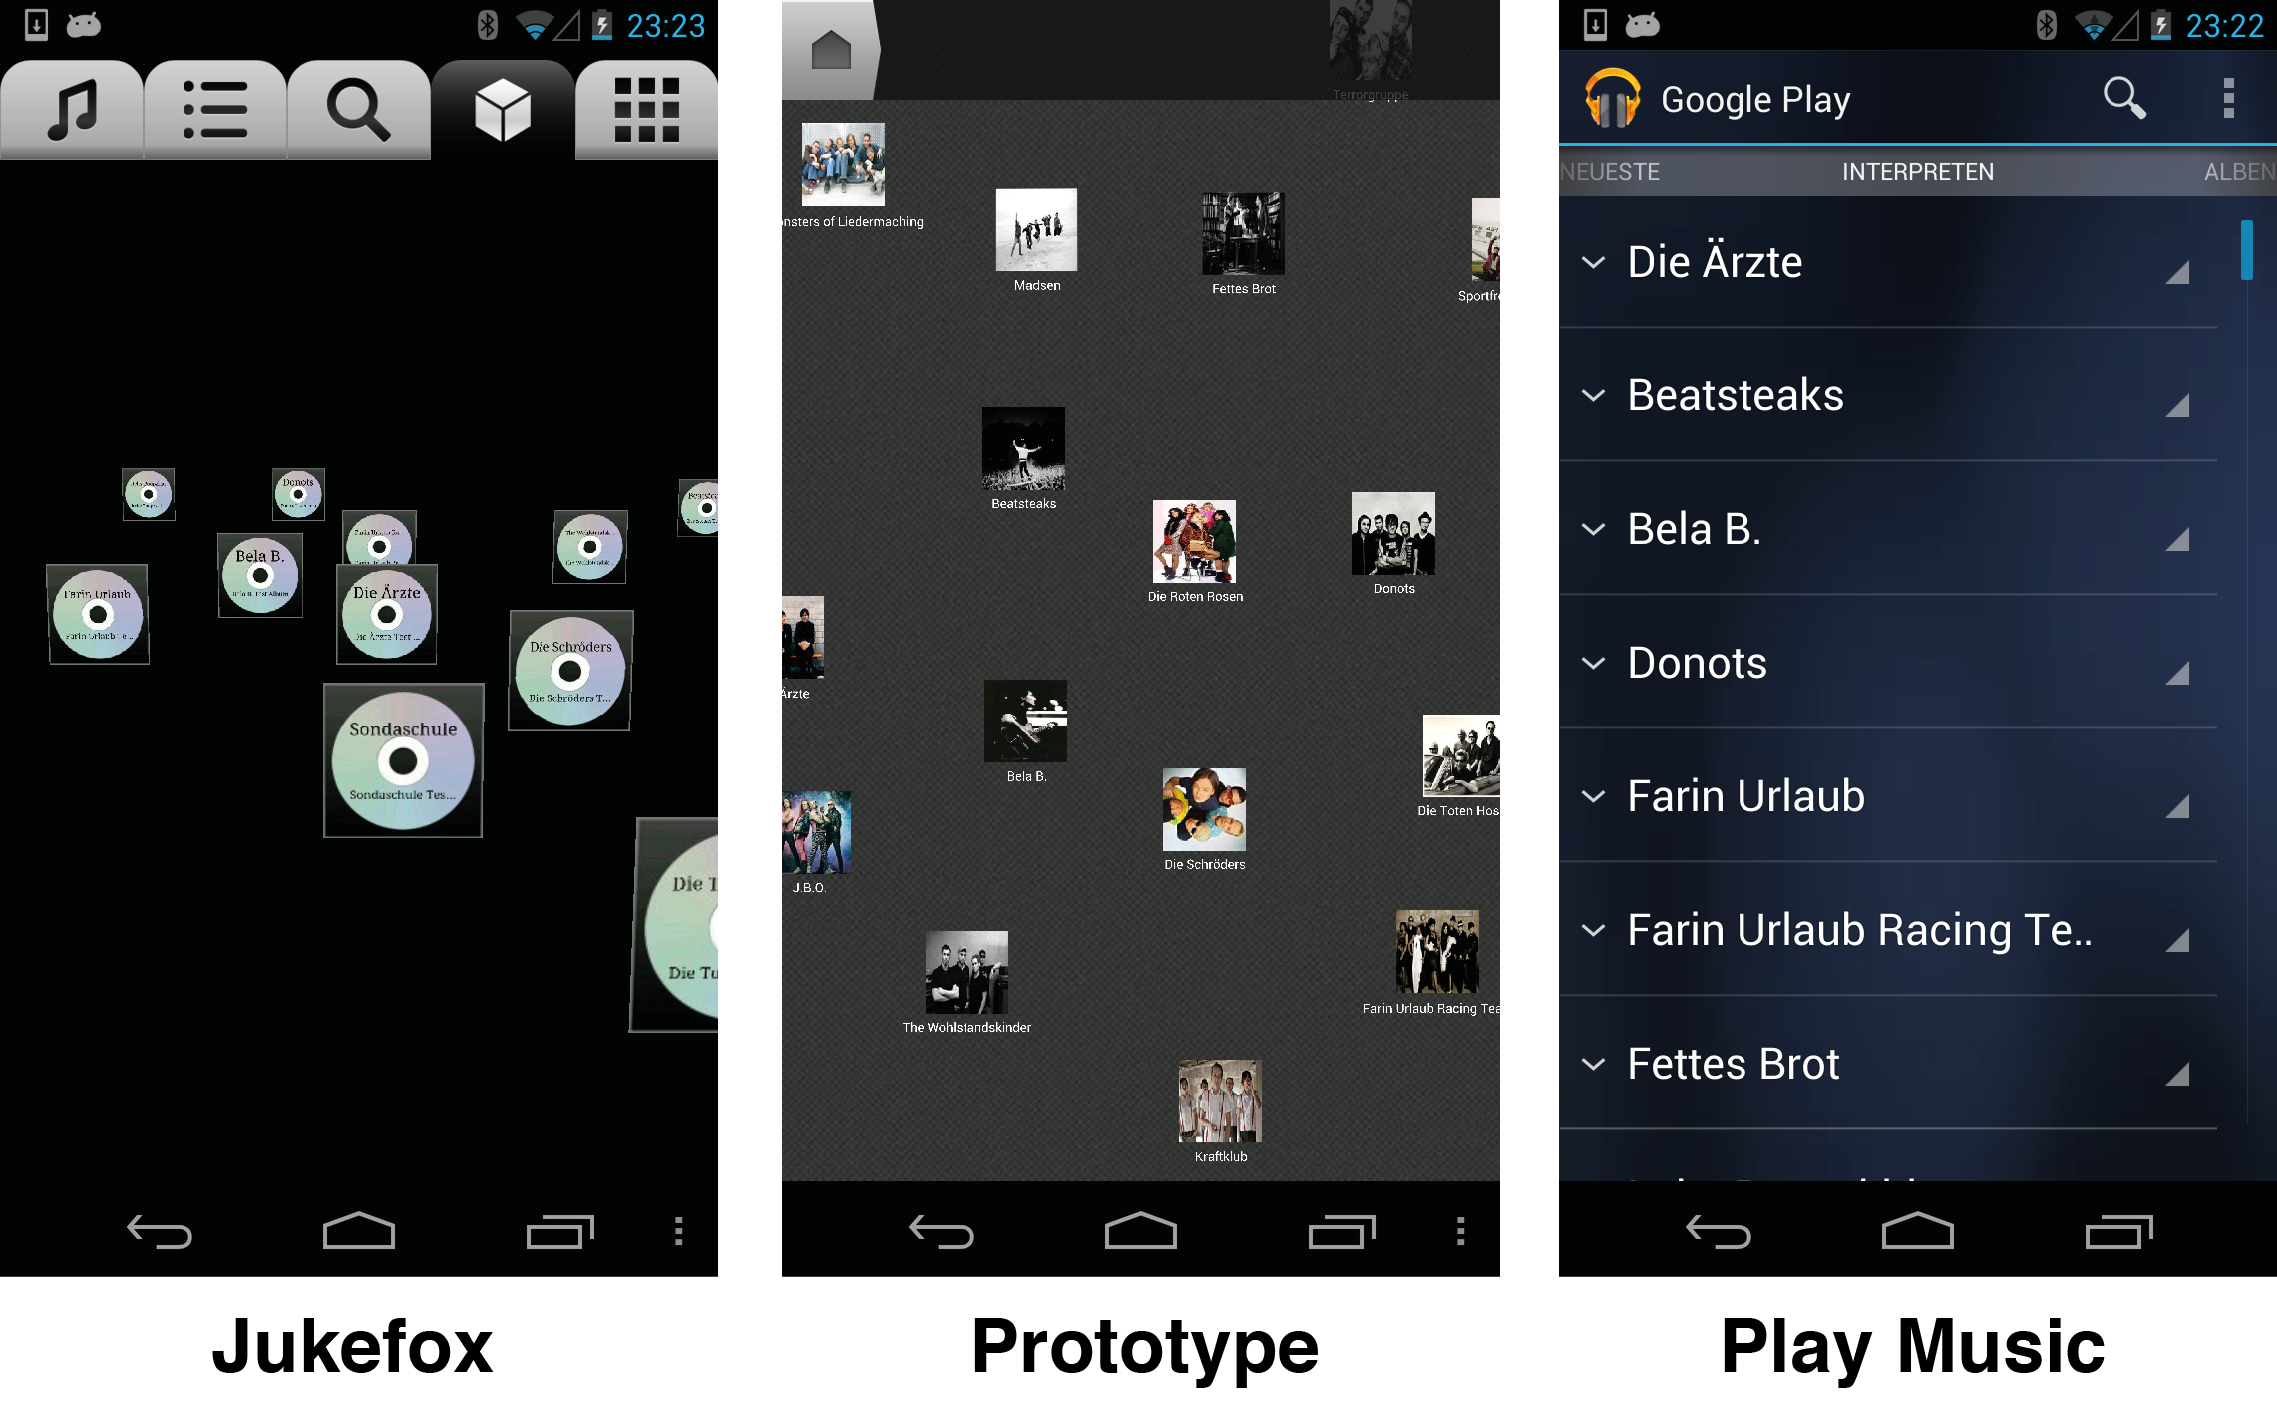
\includegraphics[width=1\textwidth]{figures/apps_screenshots}
  \caption{Screenshots of All Tested Apps}
  \label{fig:apps_screenshots}
\end{figure}

\subsection{AttrakDiff 2}

AttrakDiff 2 \cite{tubiblio21687} is a method to measure attractiveness of software to its users. It originates from the domain of user experience and is based on observations in psychology \cite{DBLP:journals/ijhci/Hassenzahl01}. AttrakDiff measures hedonic and pragmatic quality of a product, which assesses its luxurious or stimulating vs purely functional aspects. These qualities are important from a user perspective, as the perceived quality and functionality of a product can have an impact on how many users will use it for how often, or whether any people will use it at all.

Measuring the hedonic and pragmatic qualities of Andromeda will provide no isolatable statements about the usefulness of the abstract main topic of this thesis (visualization of artist similarity). But, it will give a hint of how well Andromeda resonates with users' usage patterns and aesthetic taste. The concrete questionnaire can be found in appendix ~\ref{app:attrakdiff}.

\subsection{System Usability Scale}

The System Usability Scale (SUS) has been introduced in 1986 and consists of 10 strong statements, to which a test person agrees or does not agree \cite{Lewis:2009}. Agreement or disagreement is expressed through a scale from 1 to 5. By subtraction of 1 and multiplication by 2,5, the maximum sum of all items is normalized to 100. The outcome of such an evaluation is a measure for the tested system's general usability.

Similar to AttrakDiff 2, this measure is not representative of the visualization method alone, but of Andromeda as a whole. The concrete questionnaire can be found in appendix ~\ref{app:sus}.

\subsection{Pre- and Post-Testing Questionnaires}

To find out about personal facts and opinions of the test users, questionnaires before and after the other evaluations ask for certain information. The Pre-Testing Questionnaire asks for general personal data, like age, profession, and self-assessments concerning usage of music software, while the Post-Testing Questionnaire asks for impressions of Andromeda. This data helps to put the test results into context, regarding the user demography and emotional attitude towards Andromeda. The concrete questionnaires can be found in appendices ~\ref{app:pretest} and ~\ref{app:posttest}.

\section{Population, Setup, and Process}

In the following, the setup and process of the user testing process will be described.

\begin{itemize}
  \item The study is performed with a sample of \textbf{10 test users}. 
  \item The testing takes place in a well-lit room with low noise level.
  \item Each testing takes place in one single session.
  \item Each testing consists of the following steps:
	\begin{itemize}
		\item Introduction by the tester
		\item Pre-Testing questionnaire is filled out by the test person
		\item Task-based evaluation is performed in a strict order, under close observation of the tester
		\item AttrakDiff 2 questionnaire is filled out by the test person	
		\item System Usability Scale questionnaire is filled out by the test person	
		\item Post-Testing questionnaire is filled out by the test person
	\end{itemize}
\end{itemize}

\subsection{Task-Based Evaluation Details}
\label{subsec:task-based-evaluation}

As mentioned previously, the comparison of visualization methods can be done by letting test users perform tasks, and compare how they interact with each visualization. 

This evaluation will make use of different music collections:

\begin{itemize}
	\item \textbf{One personalized collection for every user}, based on her favorite artist as a seed and all other artists being derived from a list of the most similar to the seed artist. Each test user's list was created by first asking the test user for her favorite artist (seed artist), then querying Last.fm for the 20 most similar artists of this seed artist, generating short music files (with meaningless bitstream content) with corresponding metadata, and storing the generated files in the device's media storage. The Android OS subsequently scanned the files and updated its internal music metadata caches, which are then used by all four apps under test. The rationale for this process is that this collection will likely contain mainly artists the user is familiar with, making it easier to form a mental model of the respective collection. The test tasks performed with these personalized music collections also depend on the user's rough knowledge of the contained artists (like selecting artists for a given mood).
	\item \textbf{Four predefined music collections} which contain artists which ideally are not known to the user (but knowledge of these artists has not been checked for the users, because this would skew the results). These are only used for memorization testing. Obviously, it would not do to use a personalized collection for memorization tasks, because memorization results would else be more likely to be skewed if the user knows many of the artists.
\end{itemize}

In the following, the test tasks and their metrics are listed. 


\subsubsection{Memorization}

The user shall memorize as many artists in a random music collection as possible. She is given 1 minute to do that. This test is repeated for every visualization method, and for each method a completely different music collection is loaded.

\textbf{Music Collections}: Uses the four predefined music collections, one for each visualization method.

\textbf{Metric}: Number of correctly memorized artists for each visualization method.

	
\subsubsection{Search for a Given Artist}
	
The user is asked to search for a given artist by the artist's name, without using the apps' search functionalities. This test is repeated for every visualization method.

\textbf{Music Collections}: Uses the four predefined music collections, one for each visualization method. 

\textbf{Metric}: Duration of the user's search.
	
	
\subsubsection{Recover a Given Artist After Closing the App}
	
The user is pointed to a certain artist in the music collection. Then, the app is restarted and the user has to point out the same artist again, without using the apps' search functionalities. This test is repeated for every visualization method.

\textbf{Music Collections}: Uses the four predefined music collections, one for each visualization method. 

\textbf{Metric}: Duration of the user's search after the app was restarted.
	
	
\subsubsection{Search for a Similar Artist}

The user will search visually for an artist in the presented music collection, without using the apps' search functionalities. This artist is the next-similar to the users's personalized collection's seed node (favorite artist), according to data from Last.fm. This test is repeated for every visualization method.

\textbf{Music Collections}: Uses the user's personalized music collection, based on her favorite artist as a seed.

\textbf{Metric}: Duration of the user's search.

	
\subsubsection{Search for Artists Given a Mood}
	
The user is asked to presume that she is in a certain mood. Given that mood, she has to point out 3 artists matching it. This test is repeated for every visualization method.
	
\textbf{Music Collections}: Uses the user's personalized music collection, based on her favorite artist as a seed.
	
\textbf{Metric}: Duration of the user's search for all three artists.


\section{Results and Data}

All test persons were able to understand the tasks which were asked of them. Also, all of them were able to interact with all of the tested apps. This is mostly due to the fact that every test participant has owned or at least tested a smartphone before, and multitouch gestures seems to have become a generally understood convention.

3 test persons did not know what to make of the first attributes of the AttrakDiff 2 questionnaire ("'Harmless"' vs. "'Challenging"'), and 2 test persons noted that the AttrakDiff 2 attributes "'Brings me closer to people"' vs. "'Separates me from people"' do not make sense in the context of Andromeda, because it's no social app. The observer of the tests in these cases told test users to restrict their judgements to Andromeda alone, and use a neutrally positioned option when in doubt.

Whenever objections or suggestions for improvement were mentioned during the tests, the test observer wrote them down and reminded test persons of them after the tests, so they could write them into the questionnaires if suitable.

\subsection{Study Population}

The population of the user study is characterized by an age range of [20..25] and one outlier of an age of 60 years, and the following professions:

\begin{itemize}
	\item Student at age 25, female
	\item Constructing Engineer at age 60, male
	\item Student at age 25, male
	\item Student at age 24, female
	\item Retiree at age 60, female
	\item Software Engineer at age 26, male
	\item Student at age 26, male
	\item Pupil at age 23, male
	\item Entrepreneur at age 29, male
	\item Housewife at age 24, female
\end{itemize}

In the following, statistical standard metrics are presented for most of the known attributes of test users.

\begin{table}[H]
\begin{center}
\begin{tabular}{ | c | c | }
	\hline
	\textbf{Male (\%)} & \textbf{Female (\%)} \\ \hline
	6 (60\%) & 4 (40\%) \\ \hline
\end{tabular}
\caption {Gender Distribution} \label{tab:gender} 
\end{center}
\end{table}

\begin{table}[H]
\begin{center}
\begin{tabular}{ | c | c | c | c | }
	\hline
	\textbf{Mean} & \textbf{Median}\\ \hline
	32,2 & 25,5 \\ \hline
\end{tabular}
\caption {Age Distribution} \label{tab:age-distribution} 
\end{center}
\end{table}

\begin{table}[H]
\begin{center}
\begin{tabular}{ | l | c | c | }
	\hline
	\textbf{Metric} & \textbf{Yes (\%)} & \textbf{No (\%)} \\ \hline
	Owns a Smartphone & 9 (90\%) & 1 (10\%) \\ \hline
	Has Used Desktop Music Software & 10 (100\%) & 0 (0\%) \\ \hline
	Has Used Mobile Music App & 8 (80\%) & 2 (20\%) \\ \hline
\end{tabular}
\caption {Usage Experiences} \label{tab:usage-experiences} 
\end{center}
\end{table}

\begin{table}[H]
\begin{center}
\begin{tabular}{ | l | c | c | c | c |}
	\hline
	\textbf{Metric} & \textbf{Daily (\%)} & \textbf{Weekly (\%)} & \textbf{Monthly (\%)} & \textbf{Rarely(\%)}\\ \hline
	Desktop Music Software Usage & 4 (40\%) & 6 (60\%) & 0 (0\%) & 0 (0\%) \\ \hline
	Mobile Music App Usage & 1 (10\%) & 5 (50\%) & 1 (10\%) & 3 (30\%) \\ \hline
\end{tabular}
\caption {Usage Patterns} \label{tab:usage-patterns} 
\end{center}
\end{table}

\subsection{Task-Based Evaluation Results}
\label{sec:taskbased-evaluation-results}

As all test users were asked to perform the pre-defined test tasks, a set of 10 data samples (questionnaires filled out by all participants) was gathered for each task and for each visualization. In the following tables, appropriate metrics derived from the raw data logs are shown. The top values are marked as bold. An interpretation of these test metrics will now be given. 

In table ~\ref{tab:memorization}, it can be observed that the modified Andromeda prototype with random layout performed the best (mean of 6,4 memorized artists) - users could memorize the most artists when using this app. Its performance is closely followed by the original Andromeda prototype with spring model layout. The performance difference between the two Andromeda versions is very small and can be considered insignificant, hinting to an equality of memorization performance.

Table ~\ref{tab:search-for-given} shows that test users needed considerably more time to find artists with the  "'Jukefox"' app than with any other tested app (yet, the standard deviation of 12,9 shows that search times were not homogeneous with Jukefox). Also by a large margin, the "'Play Music"' app allowed users to search in less time than the two Andromeda versions (with a mean of only 2,4 seconds per search). It is clear that Andromeda did not fare especially well, but also not especially bad in the task "'Search for a Given Artist"'.

The table ~\ref{tab:refind-given} shows that recovering an artist (i.e. searching for the same artist who was searched for in the previous task and table) in the "'Jukefox"' performed worse than the other tested apps, by a huge margin (with a mean of 9,8 seconds per artist recovery). Again, the standard deviation for Jukefox's perfomance is elevated at 4,1, telling that not all users performed approximately equal in this task. Also, "'Play Music"' again provided for the lowest search/recovery time (with 1,8 seconds per recovery), but both versions of the Andromeda app performed only slightly worse (with 2,8 and 3,5 seconds, respectively; the difference can again be viewed as insignificantly small).

In ~\ref{tab:search-similar} it can be seen that the "'Jukefox"' app again took users longest to search (mean of 14,1 seconds per search), while "'Play Music"' and the unmodified Andromeda prototype performed very similar, judging only by the mean values of 3,9 and 3,8 seconds respectively. However, "'Play Music"''s search durations feature a significantly higher standard deviation, hinting to outliers which are responsible for the result. The median values of these two apps show that "'Play Music"' (median of 1,5 seconds as opposed to a median of 3,5 seconds for unmodified Andromeda) seemed to perform better for most test users than Andromeda. The difference of 1,2 seconds between the means of the modified (randomized) and unmodified Andromeda prototypes could mean that the unmodified (spring model) prototype version performs better, but this cannot be determined at this time.

Finally, in table ~\ref{tab:search-mood}, the "'Play Music"' and both Andromeda versions performed similarly, with similar means of 16,1, 17,8, and 18,8 seconds, and medians of 16,5, 16,5, and 19 seconds. The search for three artists based on a predetermined mood seems to yield similar durations for these three apps. Only the "'Jukefox"' app again featured significantly longer search times, with a mean of 38 seconds. 
 

\begin{table}[H]
\begin{center}
\begin{tabular}{ | l | c | c | c | c |}
	\hline
	\textbf{Visualization} & \textbf{Mean} & \textbf{Median} & \textbf{Variance} & \textbf{Standard Deviation}\\ \hline
	Andromeda, Random Layout & \textbf{6,4} & \textbf{6,5} & 2,0 & 1,4 \\ \hline
	Andromeda, Similarity & 6,1 & 6,0 & 2,7 & 1,6 \\ \hline
	Play Music & 5,0 & 5,0 & 1,8 & 1,3 \\ \hline
	Jukefox & 4,2 & 4,0 & \textbf{0,6} & \textbf{0,7} \\ \hline
\end{tabular}
\caption {Memorization (Metric: Number of Memorized Artists within 30 seconds)} \label{tab:memorization} 
\end{center}
\end{table}

\begin{table}[H]
\begin{center}
\begin{tabular}{ | l | c | c | c | c |}
	\hline
	\textbf{Visualization} & \textbf{Mean} & \textbf{Median} & \textbf{Variance} & \textbf{Standard Deviation}\\ \hline
	Andromeda, Random Layout & 8,0 & 6,5 & 25,8 & 5,1 \\ \hline
	Andromeda, Similarity & 7,5 & 6,0 & 39,9 & 6,3 \\ \hline
	Play Music & 2,4 & 2,0 & \textbf{0,6} & \textbf{0,8} \\ \hline
	Jukefox & \textbf{21,9} & \textbf{18,0} & 167,5 & 12,9 \\ \hline
\end{tabular}
\caption {Search for a Given Artist (Metric: Search Duration in Seconds)} \label{tab:search-for-given} 
\end{center}
\end{table}

\begin{table}[H]
\begin{center}
\begin{tabular}{ | l | c | c | c | c |}
	\hline
	\textbf{Visualization} & \textbf{Mean} & \textbf{Median} & \textbf{Variance} & \textbf{Standard Deviation}\\ \hline
	Andromeda, Random Layout & 3,5 & 3,0 & 1,1 & 1,1 \\ \hline
	Andromeda, Similarity & 2,8 & 2,5 & \textbf{1,1} & \textbf{1,0} \\ \hline
	Play Music & 1,8 & 1,5 & 1,4 & 1,2 \\ \hline
	Jukefox & \textbf{9,8} & \textbf{8,5} & 17,2 & 4,1 \\ \hline
\end{tabular}
\caption {Recover a Given Artist (Metric: Search Duration in Seconds)} \label{tab:refind-given} 
\end{center}
\end{table}

\begin{table}[H]
\begin{center}
\begin{tabular}{ | l | c | c | c | c |}
	\hline
	\textbf{Visualization} & \textbf{Mean} & \textbf{Median} & \textbf{Variance} & \textbf{Standard Deviation}\\ \hline
	Andromeda, Random Layout & 5,0 & 4,0 & 4,6 & 2,1 \\ \hline
	Andromeda, Similarity & 3,8 & 3,5 & \textbf{2,5} & \textbf{1,6} \\ \hline
	Play Music & 3,9 & 1,5 & 45,6 & 6,8 \\ \hline
	Jukefox & \textbf{14,1} & \textbf{15,0} & 43,7 & 6,6 \\ \hline
\end{tabular}
\caption {Search for an Artist Similar to a Given One (Metric: Search Duration in Seconds)} \label{tab:search-similar} 
\end{center}
\end{table}

\begin{table}[H]
\begin{center}
\begin{tabular}{ | l | c | c | c | c |}
	\hline
	\textbf{Visualization} & \textbf{Mean} & \textbf{Median} & \textbf{Variance} & \textbf{Standard Deviation}\\ \hline
	Andromeda, Random Layout & 18,8 & 19,0 & 86,4 & 9,3 \\ \hline
	Andromeda, Similarity & 17,8 & 16,5 & 73,0 & 8,5 \\ \hline
	Play Music & 16,1 & 16,5 & \textbf{51,3} & \textbf{7,2} \\ \hline
	Jukefox & \textbf{38,0} & \textbf{41,5} & 130,8 & 11,4 \\ \hline
\end{tabular}
\caption {Search for 3 Artists Given a Certain Mood (Metric: Search Duration in Seconds)} \label{tab:search-mood} 
\end{center}
\end{table}


\subsection{Qualitative Questionnaire Results}
\label{sec:qualitative-questionnaire-results}

As mentioned before, every test participant also filled out an AttrakDiff 2 questionnaire to evaluate the unmodified Andromeda App's hedonic and pragmatic usability quality. In order to correctly interpret the test, negative attribute values are inverted, such that each attribute has a range of 1 to 7 points, where lower means better. The outcome of this test (sum of all points for each user) is  summarized by the concrete metrics derived from its evaluation in table ~\ref{tab:attrakdiff}. The pragmatic quality mean of 2,07 hints to a high usability of Andromeda, and the relatively low standard deviation of 0,53 confirms that this finding is consistent for all users. However, the hedonic quality (both identity and stimulation parts) features higher means and medians than the pragmatic quality. The interpretation of these values is that while the pragmatic (purely feature-based) quality of Andromeda is fairly good, while the hedonic (decorating) quality is not as high and should later on be improved to at least match the pragmatic quality (by adding features to Andromeda which reportedly improve this metric).

\begin{table}[H]
\begin{center}
\begin{tabular}{ | l | c | c | c | c |}
	\hline
	\textbf{Quality Metric} & \textbf{Mean} & \textbf{Median} & \textbf{Variance} & \textbf{Standard Deviation}\\ \hline
	Hedonic Quality - Stimulation & 2,54 & 2,5 & 0,29 & 0,54 \\ \hline
	Hedonic Quality - Identity & 2,69 & 2,5 & 0,27 & 0,52 \\ \hline
	Pragmatic Quality & 2,07 & 2,0 & 0,28 & 0,53 \\ \hline
\end{tabular}
\caption {The Prototype's AttrakDiff 2 Qualities on a Scale From 1-7 (Lower is Better)} \label{tab:attrakdiff} 
\end{center}
\end{table}

In order to get a grasp of the overall usability of Andromeda, each test person was also asked to fill out the system usability scale questionnaire after the AttrakDiff 2 test. In table ~\ref{tab:sus}, statistical characteristics of the SUS results are presented. The mean value of 86 for system usability scale is not homogeneous for all users, judging by the standard deviation of 8,7. The author of this thesis considers a mean of 86 as "'good enough"' in order to not disturb the user's experience during the tests, meaning the test results were most likely not skewed by a sup-par usability.

\begin{table}[H]
\begin{center}
\begin{tabular}{ | l | c | c | c | c |}
	\hline
	\textbf{Mean} & \textbf{Median} & \textbf{Variance} & \textbf{Standard Deviation}\\ \hline
	86 & 86,3 & 75,3 & 8,7 \\ \hline
\end{tabular}
\caption {Andromeda's System Usability Scale Results on a Scale from 0 - 100 (Higher is Better)} \label{tab:sus} 
\end{center}
\end{table}


\subsection{Post-Test Questionnaire Results}

All users filled out the post-test questionnaire which evaluated their impressions and hypothetical usage of Andromeda (both similarity-based and randomized layout). In tables ~\ref{tab:problems-during-testing} (how many users were experiencing problems during the tests) and ~\ref{tab:hypothetical-prototype-usage} (users answered whether or not they would use the unmodified Andromeda app in day-to-day life), two features gathered by these questionnaires are presented.

\begin{table}[H]
\begin{center}
\begin{tabular}{ | c | c | }
	\hline
	\textbf{Yes (\%)} & \textbf{No (\%)} \\ \hline
	2 (20\%) & 8 (80\%) \\ \hline
\end{tabular}
\caption {Users with Problems during the Testing} \label{tab:problems-during-testing} 
\end{center}
\end{table}

\begin{table}[H]
\begin{center}
\begin{tabular}{ | l | c | c | c | c |}
	\hline
	\textbf{Yes} & \textbf{Quite Sure} & \textbf{Rather Not} & \textbf{No}\\ \hline
	6 & 4 & 0 & 0 \\ \hline
\end{tabular}
\caption {Hypothetical Real-Life Usage of Andromeda} \label{tab:hypothetical-prototype-usage} 
\end{center}
\end{table}

\textbf{Hypothetical Usage Contexts}

Test participants were asked to list contexts where they would use Andromeda. This listing contains a compilation of the given statements:

\begin{itemize}
	\item Inspiration
	\item At home
	\item Public transit, commute, or en route
	\item Parties
	\item Search new artists
\end{itemize}

\textbf{What Users Would Change}

Test participants gave the following suggestions for Andromeda:

\begin{itemize}
	\item Font size is too small
	\item Add mood clouds
	\item Add alphabetical sorting
	\item Zooming is too fast
	\item Search new artists
\end{itemize}

\section{Observations During the Tests}

Most of the test tasks ran without any comments of the test persons - mainly due to the extensive introduction and short, concise test tasks which did not leave much room for uncertainty. In cases where searching took especially long (most of the times, with the app "'Jukefox"'), the test users observed that the interface in use was confusing, but eventually always managed to perform the task as defined without any help from the observer. As mentioned previously, two test persons had issues (and also mentioned them on the post-test questionnaire): one observed that Andromeda's font size was "'too small"', and the other person observed that the zooming was "'not intuitive"'. These issues should be investigated further in future research. Since 9 out of the 10 test users own a smartphone (and the 10th person has used smartphones before), there were no questions about touch interaction or general usage of the test device.

\section{Analysis and Discussion}

It is common for user studies with huge samples of hundreds or thousands of participants to analyze the captured raw data with stochastic tools, in order to establish certain truths and accept or reject hypotheses defined up front. A common method is to employ a T-test (Student or Welch) in order to determine whether two data sets have the same mean, with a certain confidence. A typical scenario in the context of the study discussed in this Chapter would be to find out whether it took participants less time to search for a similar artist in the similarity-based Andromeda prototype as opposed to searching for it in the randomized prototype visualization. This could be done by establishing that search times follow a normal distribution and perform a T-test for the means of the search time samples from the two prototype versions.

However, the sample for this study was made up of only 10 participants (as required by time and resource constraints) - stochastic analysis would still be possible, but the results' significance and probability of rejection of the tested null-hypotheses would be too low to provide any useful insights. For example, the above scenario of searching for a similar artist, using a two-tailed Student's T-test with a significance level of 0.2 (which is already unusually high) would only yield a 55\% probability of the alternative hypothesis being true (meaning, that the similarity-based prototype performs better). Therefore, the author will in the following discuss the study's findings in an informal way, giving insights and pointing out data points of interest.

Generally speaking, the prototype app performed well in certain areas (memorizing and searching), as expected. The Google Play music app, which was used to test a simple test-based list layout without artwork, performed considerably better in other areas, especially when searching for artists by name. Intuitively, this was to be expected because the user can parse all artists with much less scrolling, and elements are very linearly aligned.

In the following, the five hypotheses listed at the beginning of this Chapter will be discussed with the findings from the study's task-based experiments (as mentioned before, this is rather a discussion and not a stochastically supported evaluation).
The first hypothesis, \textbf{H1} (users can memorize more content using the prototype app, demonstrating a more detailed mental model of the music collection), seems to be \textbf{supported} by the study's results. As can be seen in Section ~\ref{sec:taskbased-evaluation-results}, both the randomized and similarity-based layout algorithms outperformed the other two visualization methods. This has to be due to the mode of visual representation of artists which both Andromeda versions use - both Andromeda versions have yielded almost equal memorization metrics (as mentioned previously). Since the app "'Jukefox"' also provides object-based, spatial artist representation, and users' memorization performance was poorer with this app, it can be deducted that not every object-based visualization has a positive impact on mental model forming.

Hypothesis \textbf{H2} (users can find a certain artist faster using the prototype app) does \textbf{not receive much support} from the study. While test participants were much quicker at solving the task while using any Andromeda version compared to the "'Jukefox"' app, the "'Google Play"' visualization fared best. It can be concluded that pure text-based lists are better suited for searching artists by name, than objectifying visualizations. Also, discoverability is not only dependent on the visualization paradigm (list-based vs. object-based), but is also influenced by the concrete implementation of the visualization ("'Andromeda"' vs "'Jukefox"' visualization implementation).
 
The third hypothesis, \textbf{H3} (users can recover a certain artist faster after the app was closed), is in its proposition very similar to H2. Hence, the test metrics affecting H3 are similar to the metrics affecting H2, hinting at the \textbf{refusal} of H3. The rationale behind H3 is that a spatial arrangement of artist objects (as Andromeda does) lets users recover a certain artist faster than the first time they searched for it. This was the case for the study experiments within the context of each app, but the learning effect was very strong for each app - users often found an artist in "'Google Play"' again within only 1 second, because they had only to scroll down some lines. For all apps, the mean search duration for an artist was reduced by over 50\% when the user had searched for this artist before.

\textbf{H4} (users can find the artist most similar to a seed artist faster using  similarity-based Andromeda) seems to be \textbf{refused} by the study's gathered data, similar to H2 and H3. The mean of the corresponding search duration logs indicates that the similarity-based Andromeda is on par with "'Google Play"' in this regard, but this is greatly owed to a spike caused by test person 5 - this fact is exposed when comparing the durations median (3.5 seconds for similarity-based Andromeda, 1.5 seconds for "'Google Play"'), where the latter clearly fared better. Similarity-based Andromeda seems to perform slightly better here than Andromeda with randomized layout, but this could also be due to chaos or learning effects.

The experiments did not give a clear hint of acceptance or refusal of the fifth hypothesis, \textbf{H5} (users can find 3 artists they connect to a predefined mood faster using similarity-based Andromeda). In the tests, users had to point out 3 artists which they connect with a certain mood, where the mood was determined up front for each tested app. For each tested app, one of these moods was randomly selected for the search of 3 artists: happiness, sadness, rage, and boredness. The music collection in which this mood search was performed was the respective user's personalized collection (as described in Section ~\ref{subsec:task-based-evaluation}), so each user supposedly was familiar with the contained artists. During the tests, each mood search for 3 artists completed without issues, yielding different search durations for every test user and app. "'Google Play"' performed slightly better regarding the average (mean) task duration, but is on par with similarity-based Andromeda when looking at the search duration median. Similarity-based Andromeda fared about 15\% better than randomized Andromeda w.r.t. the mean duration, but as for H4, this is \textbf{no strong enough hint} to conclude that the similarity-based layout gives users an advantage in this use case. The "'Jukefox"' app performed significantly worse than all other apps, as was the case with most other test tasks.

As a means of measuring the usability of Andromeda (both similarity-based and randomized layout, both of which versions were identical except for the spatial arrangement of artists), the AttrakDiff 2 and System Usability Scale questionnaire data provides interesting insights. \textbf{AttrakDiff 2} data statistics in Section ~\ref{sec:qualitative-questionnaire-results} show that Andromeda received good hedonic and pragmatic quality ratings featuring a relatively low standard deviation, with a median of 2,5 and 2,0 (out of 1 to 7), respectively. The \textbf{System Usability Scale} test results are comparably good, at a median of 86,3 (out of 0-100) with a standard deviation of 8,7. It can be concluded that Andromeda was adequately implemented so as to not distort the previously discussed test task metrics in a negative way.

It can be concluded that the implemented 2D visualization with a layout based on artist-similarity provides for the forming of better mental models of music collections than the visualizations used in common music apps.

\section{Summary}

In this Chapter, the planning and execution of a user study was described, and the study's gathered data was discussed. Five hypotheses were defined up front, and the study was designed around them, to find hints at the acceptance or refusal of the hypotheses. They center around the research objectives as defined in Chapter ~\ref{ch:scenario} and had the task of finding out how the previously built app prototype ("'Andromeda"') fares in comparison to other music collection visualizations on mobile devices. 

The study was carried out by the test participants performing tasks and filling out questionnaires before and after those tasks. The study population is made up of 10 adults of various ages and several professional backgrounds. As the population's size could not be increased considerable because of time and resource constraints, the data subsequently did not allow for reliable stochastic analysis, and therefore the results' discussion was restricted to informal analysis.

This subsequent analysis of the study's gathered data found that three hypotheses (H2 - H4) are likely to be rejected, one hypothesis (H5) seems to not receive a clear hint to acceptance or rejection, and another hypothesis (H1) is likely to be positive - thus, it seems to be the case that Andromeda allows for better memorization of artists than the other music apps, which could be a hint that users can form a more detailed mental model with Andromeda.

Finally, the discussion of qualitative questionnaires revealed that Andromeda was well recepted by the test participants, and that it is likely that no usability issues distorted the test tasks carried out during the experiments.